%%%%%%%%%%%%%%%%%%%%%%%%%%%%%%%%%%%%%%%%%
% Beamer Presentation
% LaTeX Template
% Version 1.0 (10/11/12)
%
% This template has been downloaded from:
% http://www.LaTeXTemplates.com
%
% License:
% CC BY-NC-SA 3.0 (http://creativecommons.org/licenses/by-nc-sa/3.0/)
%
%%%%%%%%%%%%%%%%%%%%%%%%%%%%%%%%%%%%%%%%%

%----------------------------------------------------------------------------------------
%	PACKAGES AND THEMES
%----------------------------------------------------------------------------------------

\documentclass{beamer}

\mode<presentation> {

% The Beamer class comes with a number of default slide themes
% which change the colors and layouts of slides. Below this is a list
% of all the themes, uncomment each in turn to see what they look like.

%\usetheme{default}
%\usetheme{AnnArbor}
%\usetheme{Antibes}
%\usetheme{Bergen}
%\usetheme{Berkeley}
%\usetheme{Berlin}
%\usetheme{Boadilla}
%\usetheme{CambridgeUS}
%\usetheme{Copenhagen}
%\usetheme{Darmstadt}
%\usetheme{Dresden}
%\usetheme{Frankfurt}
%\usetheme{Goettingen}
%\usetheme{Hannover}
%\usetheme{Ilmenau}
%\usetheme{JuanLesPins}
%\usetheme{Luebeck}
%\usetheme{Madrid}
%\usetheme{Malmoe}
%\usetheme{Marburg}
%\usetheme{Montpellier}
%\usetheme{PaloAlto}
%\usetheme{Pittsburgh}
\usetheme{Rochester}
%\usetheme{Singapore}
%\usetheme{Szeged}
%\usetheme{Warsaw}

% As well as themes, the Beamer class has a number of color themes
% for any slide theme. Uncomment each of these in turn to see how it
% changes the colors of your current slide theme.

%\usecolortheme{albatross}
%\usecolortheme{beaver}
%\usecolortheme{beetle}
%\usecolortheme{crane}
%\usecolortheme{dolphin}
%\usecolortheme{dove}
%\usecolortheme{fly}
%\usecolortheme{lily}
%\usecolortheme{orchid}
%\usecolortheme{rose}
%\usecolortheme{seagull}
%\usecolortheme{seahorse}
%\usecolortheme{whale}
\usecolortheme{wolverine}

%\setbeamertemplate{footline} % To remove the footer line in all slides uncomment this line
%\setbeamertemplate{footline}[page number] % To replace the footer line in all slides with a simple slide count uncomment this line

%\setbeamertemplate{navigation symbols}{} % To remove the navigation symbols from the bottom of all slides uncomment this line
}

\usepackage{graphicx} % Allows including images
\usepackage{booktabs} % Allows the use of \toprule, \midrule and \bottomrule in tables
%\usepackage{movie15}
%%%%% SPECIAL PACKAGES %%%%%%%%%%
\usepackage{setspace}
%\usepackage[ngerman]{babel}
\usepackage[utf8]{inputenc}
\usepackage{fancyhdr}
\usepackage{tabularx}
%\renewcommand{\rmdefault}{phv}
%\renewcommand{\sfdefault}{phv}

\setcounter{tocdepth}{2} % to get subsubsections in toc 
% cf. http://www.latex-community.org/forum/viewtopic.php?f=47&p=44760

\usepackage{amssymb,latexsym}
\usepackage{amsmath, amsthm}

%for bibliography; installation using 'sudo tlmgr install amsrefs'
\usepackage{amsrefs}

\usepackage{graphics}
\usepackage{animate}
%\usepackage{xmpmulti}

\usepackage{hyperref}
\hypersetup{colorlinks=true, urlcolor=blue}

\usepackage{cancel} % http://jansoehlke.com/2010/06/strikethrough-in-latex/

\usepackage{listings} % http://en.wikibooks.org/wiki/LaTeX/Source_Code_Listings
% http://olmjo.com/files/teaching/PSC505/LaTeXandR.pdf

% package for flower symbol (\ding(96))
\usepackage{pifont}
% required installation: sudo apt-get install texlive-fonts-recommended (30MB)
% http://tug.ctan.org/info/symbols/comprehensive/symbols-a4.pdf

\usepackage{tikz} % for diagrams
\usetikzlibrary{matrix,positioning,arrows,calc,decorations.pathmorphing,shapes}
% for snaky lines (http://tex.stackexchange.com/questions/209942/curved-arrows-in-tikz) 
\tikzset{snake it/.style={-stealth,
decoration={snake, 
    amplitude = .4mm,
    segment length = 2mm,
    post length=0.9mm},decorate}}

\usepackage[parfill]{parskip}

\usepackage{framed} %for putting some text in boxes using \begin{framed}

\usepackage{enumerate}

%for displaying tensor indices properly. requires installation of tensor package using 'sudo tlmgr install tensor'
\usepackage{tensor}

%for placing captions of figures on the side instead of above/below the figure
\usepackage{sidecap}
\linespread{1.2}

%plain makes sure that we have page numbers
%\pagestyle{plain}

\theoremstyle{plain}
\newtheorem{axiom}{Axiom}
\newtheorem*{main}{Main Theorem}
\newtheorem{proposition}{Proposition}

\theoremstyle{definition}

\theoremstyle{remark}
\newtheorem*{notation}{Notation}

\numberwithin{equation}{section}
\numberwithin{figure}{section}
\numberwithin{theorem}{section}

%symbol for maps
\renewcommand{\to}{\longrightarrow}
\newcommand{\injmapto}{\hookrightarrow}
\newcommand{\surjmapto}{\twoheadrightarrow}
\newcommand{\linearmapto}{\stackrel{\sim}{\longrightarrow}}
\newcommand{\projmapto}{\stackrel{\pi}{\longrightarrow}}

%for real numbers
\newcommand{\R}{\mathbb{R}}

% manifold, atlas and topology
\newcommand{\A}{\mathcal{A}}
%\newcommand{\O}{\mathcal{O}}
\newcommand{\mfd}{(M, \mathcal{O}, \mathcal{A})}

\newcommand{\after}{\circ}
\newcommand{\stdtop}{\mathcal{O}_{std}}
\newcommand{\cibasis}[2][]{\frac{\partial #1}{\partial #2}}

%connection coefficient functions or gammas
\newcommand{\ccf}[2]{\Gamma\indices{^{#1}_{#2}}}
\newcommand{\ccfx}[3]{\left(\Gamma_{#3}\right)\indices{^{#1}_{#2}}} % with chart index

%set theory symbols
%\renewcommand{\exists}{\exists\,}
%\renewcommand{\forall}{\forall\,}

%This defines a new command \questionhead which takes one argument and prints out Question #. with some space.
\newcommand{\questionhead}[1]
  {
   \noindent{\small\bf Question #1.}
  }

\newcommand{\problemhead}[1]
  {
   \noindent{\small\bf Problem #1.}
  }

\newcommand{\exercisehead}[1]
  { \smallskip
   \noindent{\small\bf Exercise #1.}
  }

\newcommand{\solutionhead}[1]
  {
   \noindent{\small\bf Solution #1.}
  }

\newcommand{\bubblethis}[2]{
  \tikz[remember picture,baseline]{\node[anchor=base,inner sep=0,outer sep=0](#1) {#1};\node[overlay,cloud callout,callout relative pointer={(0.2cm,-0.7cm)}, aspect=2.5,fill=white!90] at ($(#1.north)+(-0.5cm,1.6cm)$) {#2};}
}



%%%%%%%%%%%%%%%%%%%%%%%%%%%%%


%----------------------------------------------------------------------------------------
%	TITLE PAGE
%----------------------------------------------------------------------------------------
\title[LLM Survey]{LLM Survey} % The short title appears at the bottom of every slide, the full title is only on the title page

\author{Piyush Kaul} % Your name
\institute[IITD] % Your institution as it will appear on the bottom of every slide, may be shorthand to save space
{
 \\ % Your institution for the title page
\medskip
\textit{piyushkaul@ieee.org} % Your email address
}
\date{\today} % Date, can be changed to a custom date

\begin{document}

\begin{frame}
\titlepage % Print the title page as the first slide
\end{frame}

\begin{frame}
\frametitle{Overview} % Table of contents slide, comment this block out to remove it
\tableofcontents % Throughout your presentation, if you choose to use \section{} and \subsection{} commands, these will automatically be printed on this slide as an overview of your presentation
\end{frame}

%----------------------------------------------------------------------------------------
%	PRESENTATION SLIDES
%----------------------------------------------------------------------------------------

%------------------------------------------------
\section{LoRA} % Sections can be created in order to organize your presentation into discrete blocks, all sections and subsections are automatically printed in the table of contents as an overview of the talk
%------------------------------------------------


\begin{frame}
\frametitle{LoRA - Low Rank Adaptation of LLM}
Objective
\begin{enumerate}
  \item The trained LLMs are generic. Need to be fined tuned for tasks. 
  \item Not possible to train LLM without enormous amout of GPUS/Compute power.
  \item Weight changes due to fine tuning can be modelled as Low Rank layers in parallel.
  \item We only allow the added Low Rank Dcomposition layers to tain.
  \item For GPT3, 175 MB, low rank of 2 is adequate. Full rank being quite large.
\end{enumerate}
\end{frame}

\begin{frame}[shrink]
\frametitle{LoRA - Low Rank Adaptation of LLM}
For pre-trained matrix $W_0$, the augmented networks is defined as.
\begin{align}
    W_0 + \delta W = W_0 + BA
\end{align}
where $B \in R^{d \times r}$ and $A\in R^{r\times k}$
\begin{enumerate}
\item $W_0$ stays frozen whereas only B and A are trained
\item The basic model weight set $W_0$ is common across tasks and only B and A need to be switched.
\item Generalization is possible for full fine-tuning as well.
\item Only the attention weights need to be fine tuned. The MLP weight can stay frozen.
\end{enumerate}
\end{frame}

\begin{frame}
\frametitle{LoRA - Results}
\begin{enumerate}
    \item Reduce memory size by 1000 times. 350 GB $\to$ 35 MB
\end{enumerate}
\end{frame}


\begin{frame}
\frametitle{LoRA - Layer Decomposition}
\begin{figure}
    \centering
    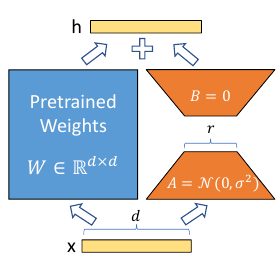
\includegraphics[width=0.5\linewidth]{lora.png}
    \caption{Enter Caption}
    \label{fig:enter-label}
\end{figure}
\end{frame}


\begin{frame}
\frametitle{QLoRA: Efficient Finetuning of Quantized LLM}
QLoRA reduces memory requirement from $>$ 700 GB of GPU to <48 GB
Following advantages are mentioned
\begin{enumerate}
    \item 4-bit Normal Float. Better than 4-bit integer and 4-bit float
    \item Double Quantization. Quantizing Quant info (saving of approx 3GB for 65 GB)
    \item Paged Optimizers. Avoid gradient checkpointing spikes.
\end{enumerate}
\end{frame}
Additional points

\section{QLoRA}
\section{ZeroQuant-FP}
\section{GPTQ}
\section{Optimal Brain Compression}


%------------------------------------------------

\begin{frame}
\frametitle{References}
\footnotesize{
\begin{thebibliography}{99} % Beamer does not support BibTeX so references must be inserted manually as below
\bibitem[Schuller, 2012]{p1}  Fredric Schuller(2012)
\textit{Lectures on Geometrical Anatomy of Physics}
%\verb{https://www.youtube.com/watch?v=V49i_LM8B0E}

\bibitem[Isham, 1989]{p2} Chris Isham(1989)
\textit{ Modern Differential Geometry for Physicists}

\bibitem[Nash, 1989]{p3} Charles Nash(2011)
\textit{ Topology and Geometry for Physics }

\bibitem[Nakahara, 2003]{p4} Mikio Nakahara(2003)
\textit{ Geometry, Topology and Physics}

\end{thebibliography}
}
\end{frame}

%------------------------------------------------

\begin{frame}
\Huge{\centerline{The End}}
\end{frame}

%----------------------------------------------------------------------------------------

\end{document} 